\documentclass{standalone}
\usepackage{tikz}
\usetikzlibrary{positioning,calc}
\usepackage{amsmath}  

\begin{document}
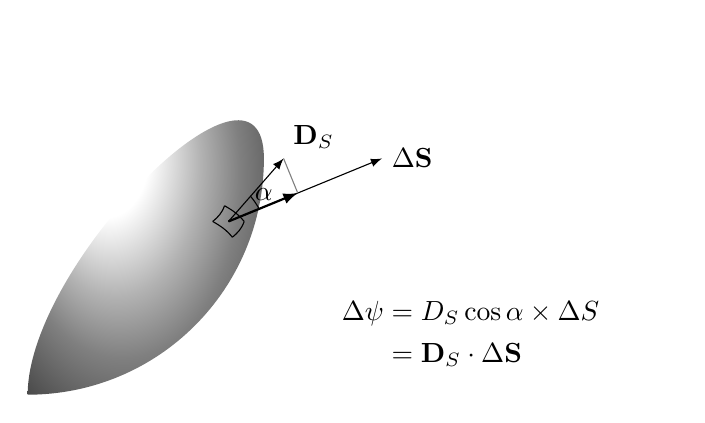
\begin{tikzpicture}
%\draw[gray,step=1](0,0) grid(5,4);
%large volume
\shade[ball color=white] (0,0) to [out=0,in=270] (3,3) to [out=90, in=90] (0,0);
%small area
\draw (2.5,2.4) to [out=330,in=130] (2.75,2.2);
\draw (2.35,2.2) to [out=330,in=130] (2.6,2) ;
\draw (2.5,2.4) to [out=250,in=40] (2.35,2.2) ;
\draw (2.75,2.2) to [out=250,in=40] (2.6,2) ;
%vectors
\draw[-latex](2.55,2.2)--(4.5,3) node[right] {$\Delta \bf{S}$};
\draw[-latex](2.55,2.2)--(3.25,3)node[above right] {${\bf{D}}_S$};
\draw[-latex,thick] (2.55,2.2)--($(2.55,2.2)!(3.25,3)!(4.5,3)$);
%perpendicular
\draw[gray,thin] (3.25,3)--($(2.55,2.2)!(3.25,3)!(4.5,3)$);
%angle
\draw ($(2.55,2.2)!0.2!(4.5,3)$) to [out=120,in=310] ($(2.55,2.2)!0.4!(3.25,3)$);
\node at (3,2.54){$\alpha$};
%text
\node[right] at (3,1){
\begin{minipage}{5cm}
\begin{align*}
\Delta \psi&= D_S \cos \alpha \times \Delta S\\
&={\bf {D}}_S \cdot \Delta {\bf{S}}
 \end{align*}
\end{minipage}
 };
%\draw plot[smooth] coordinates {(4,0) (2,0) (1,0.5) (0.4,1) (0,2) (0.5,3) (1.5,3.2) (2.5,3) (2.6,2)  (3,1) (4,0)};
%\shade[rotate=30,shade,ball color=white] ellipse (3 and 2);
\end{tikzpicture}
\end{document}
